\section{Introduction and Motivation}
\label{sec:introduction}
A software \textit{bug report} is a descriptive document used to record the scenario of a software product's unexpected behaviors. It provides information for developers to find the cause, which is usually a coding mistake called \textit{bug} or \textit{defect} \cite{Bruegge:2009:OSE:1795808}. During a software product's life cycle, the development team will usually receive a large number of bug reports. For example, the Eclipse Platform project team received 1,567 bug reports in 2017 alone\footnote{https://bugs.eclipse.org/bugs/}. On the one hand, bug reports provide developers with helpful information in debugging \cite{Buse:2012:INS:2337223.2337343}, but on the other, their diversity and uneven qualities can make the bug-fixing process nontrivial \cite{Breu:2010:INB:1718918.1718973}.

Upon receiving a bug report, the assignee will usually use the report information to reproduce the problem \cite{LaToza:2010:HQC:1937117.1937125} and perform code review \cite{Bacchelli:2013:EOC:2486788.2486882} to locate the bug. This manual process can be time-consuming \cite{Murphy-Hill:2013:DBF:2486788.2486833}. To help developers alleviate such tedious effort, several Information Retrieval (IR)-based automatic approaches have recently been proposed to reduce the bug-search space from the whole source code repository, which may contain thousands of files, to a much smaller range (e.g., a list of several highly recommended files). For example, Lam et al. \cite{7372035} and Huo et al. \cite{Huo:2017:EUF:3172077.3172153, Huo:2016:LUF:3060832.3060845} use Deep Neural Networks (DNN) to learn to relate source code files to bug reports. Ye et al. \cite{Ye:ICSE16, Ye:FSE14} develope a learning-to-rank model to combine various \textit{features} for ranking source files. Sahar et al. \cite{Saha:2013:ASE:6693093} and Zhou et al. \cite{Zhou:2012:BFM:2337223.2337226} used Vector Space Model (VSM), Kim et al. \cite{Kim:2013:WFT:2554428.2554437} apply Na\"{i}ve Bayes, Nguyen et al. \cite{Nguyen:2011:TAN:2190078.2190181} and Lukins et al. \cite{Lukins:2010:BLU:1824820.1824850} use Latent Dirichlet Allocation (LDA), Rao et al. \cite{Rao:2011:RSL:1985441.1985451} apply various IR models including VSM and LDA to measure the relaitonship between bug reports and source files for recommendations.

These IR-based approaches, unlike some other specturm-based approaches \cite{Cleve:2005:LCP:1062455.1062522, Dit:2013:IIR:2436118.2436134, Poshyvanyk:2013:CLU:2377656.2377660, Poshyvanyk:2007:FLU:1263152.1263534, Liu:2005:SSM:1081706.1081753, Jin:2013:FFL:2483760.2483763, B.Le:2016:LBF:2931037.2931049, Le:2015:IRS:2786805.2786880, Jones:2005:EET:1101908.1101949} that use runtime execution information to locate bugs, do not require running test cases. However, because they rely on the bug report content, the uneven quality of bug reports can be an impediment to their performance.

According to a user study by Bettenburg et al. \cite{Bettenburg:2008:MGB:1453101.1453146}, in which they receive responses from 446 developers, there is usually a mismatch between what developers consider most helpful and what is provided in the bug reports. The quality of bug report contents can vary remarkably. Bug reports may provide insufficient or even inadequate information for developers to find the cause \cite{Bettenburg:2008:MGB:1453101.1453146, Kim:2013:WFT:2554428.2554437, Hooimeijer:2007:MBR:1321631.1321639}.

Besides, some bug reports can be helpful to developers for manual search but not for IR-based approaches. Take Eclipse bug 305571\footnote{https://bugs.eclipse.org/bugs/show\_bug.cgi?id=305571} for example, it reports a problem described as ``\textit{Links in forms editors keep getting bolder and bolder}''. It provides information to reproduce the problem. Through a serious of intra-group communications, developers reproduced the abnormal scenario, got screenshots, performed manual investigations, and eventually fixed the bug in file \textit{TextHyperlinkSegment.java}. However, this buggy file does not have explicit semantic relationship with the bug report. So when we used the Lucene\footnote{https://lucene.apache.org/core/2\_9\_4/scoring.html} implementation of VSM to rank all the source files for this report, the buggy file was ranked much lower than some irrelevant files such as \textit{FormPage.java} and \textit{FormEditor.java} that have greater lexical similarity with the report.

As such, for low-quality reports and reports that do not semantically relate to the bug, instead of running an IR-based ranking system to obtain incorrect recommendations, keeping silent can reduce false positives and increase the average ranking precision.

Kim et al. \cite{Kim:2013:WFT:2554428.2554437} proposed a two-phase model that first classifies bug reports into either ``predictable'' or ``deficient'' and then locates bugs for only ``predictable'' reports. Their model uses fixed buggy files as labels and applies Na\"{i}ve Bayes to classify a ``predictable'' report to a specific label (buggy file). However, if a new buggy file has not been fixed before, it would not be considered as a label and hence cannot not be located. Despite of this problem, Kim's work inspire us to, before applying a specific IR-based system to find the bug, perform classification to filter out deficient reports and reports that are unhelpful to the IR-based system.

This paper proposes a Long Short-Term Memory (LSTM)-based pre-filtering approach to classify bug reports as either ``predictable'' or ``unpredictable''. An LSTM network is a Recurrent Neural Network (RNN) with LSTM units \cite{Hochreiter:1997:LSM:1246443.1246450} for learning features from sequence data. It has been recently used in the Software Engineering (SE) domain to solve SE problems \cite{8255666, Huo:2017:EUF:3172077.3172153}. We use LSTM to learn from bug reports their vector representations, which are then serve as input \textit{features} to a \textit{Softmax} layer for classification. If a bug report is classified as ``predictable'', we use an existing IR-based system to help locate the bug for it, otherwise, we keep silent.

We test our classification approach over 11,000 bug reports from three large-scale open source Java projects. Experiments show that, under a trade-off between the classification recall and precision, our approach can help an IR-based bug-locating system achieve better ranking result.

We also perform evaluations to compare LSTM with Convolutional Neural Network (CNN) \cite{726791} (another class of DNN that is recently used to solve SE tasks \cite{Le:2015:IRS:2786805.2786880, Xu:2016:PSL:2970276.2970357, Mou:2016:CNN:3015812.3016002}), multilayer perceptron \cite{Hornik:1989:MFN:70405.70408}, and a simple baseline approach classifying a bug report based on its length with the assumption that larger content may contain more helpful information. Results show that the simple baseline approach can achieve comparably result with multilayer perceptron. LSTM and CNN perform better than the others. LSTM achieves the best trade-off between precision and recall. 

The main contributions of this paper include: a bug report pre-filtering model to filter out ``unpredictable'' reports before running an IR-based system for bug locating; an adaptation of LSTM in the task of bug report classification; extensive evaluations to compare the effectiveness of LSTM with CNN, multilayer perceptron, and a simple baseline approach.

The rest of this paper is structured as follows. Section 2 draws an overall picture of the pre-filtering model for bug locating. Section 3 details the adaptation of an LSTM network for bug report classification. Section 4 introduces CNN, multilayer perceptron, and a simple baseline approach used for comparisons. Section 5 presents the evaluation setup and result. Following a discussion of related work in Section 6, the paper ends in Section 7 with future work and concluding remark.

\section{High Level Architecture of Bug Report Pre-Filtering}
\label{sec:high level architecture}
\begin{figure}[t]
\centering
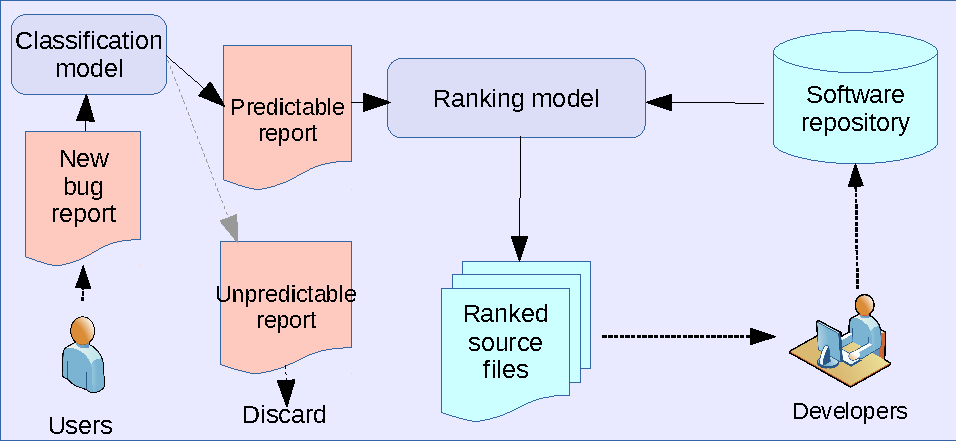
\includegraphics[width=\columnwidth]{figures/prefiltering.pdf}
\caption{High level architecture: pre-filtering before ranking.}
\label{fig:prefiltering architecture}
\end{figure}
Figure~\ref{fig:prefiltering architecture} shows the high level architecture of our bug report pre-filtering approach. When a new bug report is received, it will first be classified by a classification model into one of the two categories: ``predictable'' and ``unpredictable''. A ``predictable'' report is considered as informative and helpful to an IR-based ranking system for bug locating. It serves as input to the ranking system, which uses the report content to rank all the source code files and recommend the top ranked ones as ``buggy'' to developers to review. An ``unpredictable'' report, instead, is considered unhelpful to the IR-based ranking system and will be discarded. By keeping silent on unhelpful reports, the ranking system can reduce the number of false positives and make the recommendations be more trustworthy.

\section{Bug Report Classification using an LSTM Network}
\label{sec:lstm-based classification}
\begin{figure}[t]
\centering
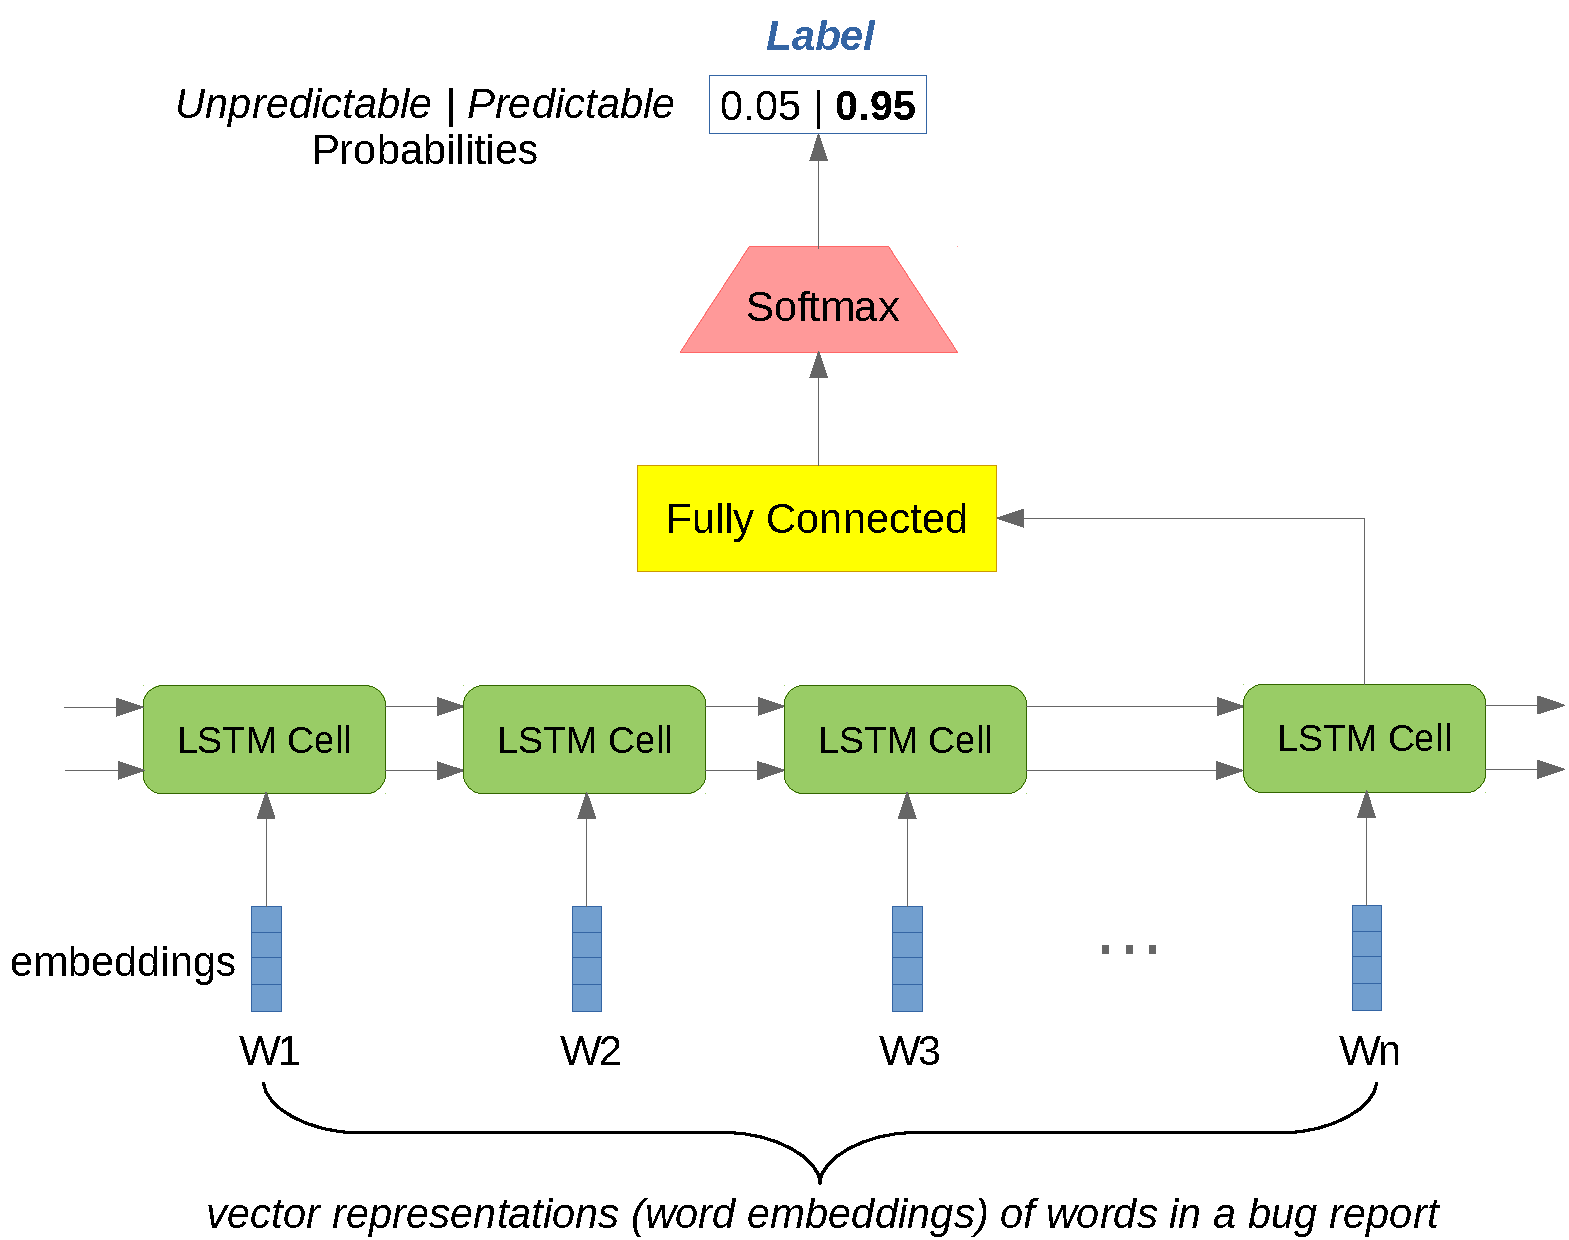
\includegraphics[width=\columnwidth]{figures/lstm.pdf}
\caption{Bug-report classification architecture: using LSTM.}
\label{fig:lstm}
\end{figure}
The architecture of the classification model is shown in Figure~\ref{fig:lstm}. Given a bug report, it takes as input the vector representations of words in the report to a Recurrent Neural Network (RNN) implemented with LSTM units. The output of the LSTM unit at the last time step is fed into a fully connected layer, followed by the Softmax model that produces the categorical distribution.

The following subsections detail each step of this process.

\subsection{From Bug Report to Bug Report Matrix}
\label{sec:bug report matrix}
Given a bug report, we concatenate its summary and its description into one document. Punctuation and numerical numbers are removed. Then we split the text by white space and obtain a bag-of-words $T$ of the document: $T = (w_1, w_2, w_3, ... w_N)$, where $w_i$ is a word token in the report and $N$ is the total number of words.

Next, we represent every word token $w_i$ with a $d$-dimensional vector of real numbers $\mathbf{w}_i$ called word embedding that captures some contextual semantic meanings \cite{NIPS2014_5477}. We use Mikolov's Skip-gram model \cite{DBLP:conf/icml/LeM14} to learn word embeddings with size of 100 on the Wikipedia data dumps\footnote{https://dumps.wikimedia.org/enwiki/}. For unseen words that are not in the Wiki vocabulary, we represent them using a vector that all 100 elements are randomly generated within the range of $(-1,1)$.

Bug reports may have different lengths. RNN can work on variable-length sequence input. However, when we train and update the LSTM network, we use multiple bug reports (e.g., 64) in a mini-batch to compute the gradient of the cost function at each step. For simplicity, we set a fixed size of 100 to all the bug reports so that a training batch can be represented by a single tensor in the TensorFlow implementation of RNN\footnote{https://www.tensorflow.org/tutorials/recurrent}. A bug report with less than 100 words will be padded with zero vectors.

Then the original bag-of-words $T$ of a bug report is converted into a matrix of real numbers: $\mathcal{M} \in \mathbb{R}^{100x100}$, where $\mathcal{M} = (\mathbf{w}_1, \mathbf{w}_2, $ \\ $\mathbf{w}_3, ..., \mathbf{w}_{100})$ and $\mathbf{w}_i \in \mathbb{R}^{100}$ is the embedding of word $w_i$. We call this matrix a bug report matrix that serves as input to the LSTM network.

\subsection{From Bug Report Matrix to Feature Vector}
\label{sec:features}
An LSTM network is a RNN using LSTM units in the hidden layer, where an LSTM unit is composed of a \textit{memory cell} and three multiplicative gates (an \textit{input gate}, an \textit{output gate}, and a \textit{forget gate}) \cite{Hochreiter:1997:LSM:1246443.1246450}. An LSTM (memory) cell $\mathbf{c}_t \in \mathbb{R}^{m}$ is a $m$-dimensional vector that stores $m$ values (states) of the hidden layer at time step $t$. The three multiplicative gates are used to control the memory of the hidden states and the update of the output. RNNs allow information (weights of connections between the input and the hidden layer) to be accumulated from previous time steps. They are powerful for modeling dependencies in time series \cite{Sutskever:2014:SSL:2969033.2969173, Goodfellow:2016:DL:3086952}. Traditional RNNs are difficulty to train on long sequence due to the vanishing gradient problem \cite{Bengio:1994:LLD:2325857.2328340}. LSTM networks effectively alleviate this problem by using the multiplicative gates to learn long-term dependencies over long periods of time.

\begin{figure}[t]
\centering
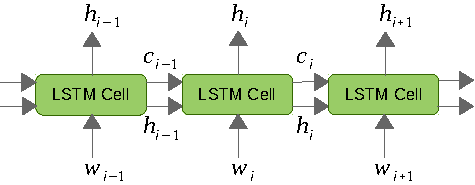
\includegraphics[scale=0.9]{figures/lstm2.pdf}
\caption{An LSTM Network.}
\label{fig:lstm2}
\end{figure}

The LSTM network takes the bug report matrix $\mathcal{M}$ as a time series input (from $\mathbf{w}_1$ to $\mathbf{w}_{100}$). At each time step, as shown Figure~\ref{fig:lstm2}, an embedding $\mathbf{w}_i$ is fed into the LSTM network, where the output $\mathbf{h}_i \in \mathbb{R}^{m}$ of an LSTM unit is determined based on three types of input: the current embedding $\mathbf{w}_i \in \mathbb{R}^{100}$, the previous LSTM output $\mathbf{h}_{i-1} \in \mathbb{R}^{m}$, and the content of the memory cell $\mathbf{c}_{i-1} \in \mathbb{R}^{m}$ from the previous time step, where $m$ is the number of hidden units (states) in the memory cell.

In this paper, the output of the LSTM unit from the last time step $\mathbf{h}_{100} \in \mathbb{R}^{m}$ is used as the final output $\mathbf{h}$ of the LSTM network. It is a feature vector representation of the original bug report that captures the structural and semantic dependencies.

\subsection{From Feature Vector to Categorical Distribution}
\label{sec:categorical distribution}
The output of the LSTM network $\mathbf{h} \in \mathbb{R}^{m}$ is fed into a fully connected layer with rectifier (ReLU) \cite{Nair:2010:RLU:3104322.3104425} activation function.

\begin{equation}
  \mathbf{x} = max(\mathbf{f}, 0), \:\:\:\:\:\: \mathbf{f} = \mathbf{U}^T \mathbf{h} + \mathbf{b}
\label{eq:fully connected}
\end{equation}

The output $\mathbf{x} \in \mathbb{R}^{n}$ of the fully connected layer is shown in Equation~\ref{eq:fully connected}, where $\mathbf{U} \in \mathbb{R}^{mxn}$ is the weighting matrix initialized using the Glorot uniform scheme \cite{DBLP:journals/jmlr/GlorotB10}, $\mathbf{b} \in \mathbb{R}^{n}$ is the bias, and $n=2$ is the number of categories. It serves as input to a Softmax model.

Softmax normalizes $\mathbf{x} \in \mathbb{R}^{n}$ into a new $n$-dimensional vector $\mathbf{\tilde{y}}$ with real numbers in the range $[0,1]$. The elements of $\mathbf{\tilde{y}}$ sum up to 1. So it can be used as the categorical (probability) distribution over all the possible categories: ``predictable'' and ``unpredictable''.

\begin{equation}
  \tilde{y_i} = P(r \in i|\mathbf{x}) = \sigma(\mathbf{v}_i^T\mathbf{x}) = {exp({\mathbf{v}_i}^T\mathbf{x}) \over \sum_{k=1}^{2}exp({\mathbf{v}_k}^T\mathbf{x})}, \:\:\:\:\:\: i \in [1,2]
\label{eq:softmax}
\end{equation}

Given $\mathbf{x}$, the probability of the $i^{th}$ category for bug report $r$ is denoted in Equation~\ref{eq:softmax}, where $\mathbf{v}$ is the weighting vector.

Finally, the bug report is classified to the category with the largest probability value.

\subsection{Model Training}
\label{sec:model training}
Parameters of the LSTM network, fully connected layer, and the Softmax model are trained on minimizing the cross-entropy error using Adam (adaptive moment estimation) optimizer \cite{DBLP:journals/corr/KingmaB14}.

\begin{equation}
  J(w) = \sum_{r \in R}\sum_{i=1}^{n}(y_i \log \tilde{y_i} + (1-y_i) \log (1-\tilde{y_i}))
\label{eq:cross entropy}
\end{equation}

The cross-entropy cost function is shown in Equation~\ref{eq:cross entropy}, where $y_i$ is the observed probability of category $i$ for bug report $r$, $\tilde{y_i}$ is the estimated probability, $R$ denotes a training batch.

Before training, the training set is split into small \textit{batches}. During training, the models are updated using the gradient of the cost function computed over a mini-batch set. Using batches improves training efficiency, helps avoid local minima, and achieves better convergence \cite{Goodfellow:2016:DL:3086952}.

One cycle (a forward pass and a backward pass) of seeing all the training data is called an \textit{epoch}. Let $T$ denotes the training set and $R$ be a mini-batch, the number of batches is $num\_batches = |T||R|^{-1}$. So each epoch updates the models $num\_batches$ times .

The models are trained over a maximum 500 epochs with an earlier stopping criterion, which deems convergence when seeing a certain number (e.g., 10) of continuous performance degrade on the validation dataset.

To achieve more robust convergence, we also apply the \textit{variational dropout} technique \cite{Gal:2016:TGA:3157096.3157211} during training, which reduces over-fittings by randomly cleaning up some input, output, and hidden units.

\section{Bug Report Classification using CNN, Multilayer Perceptron, and a Simple Baseline}
\label{sec:cnn perceptron simple baseline}
This section introduces bug report classification using Convolutional Neural Network (CNN), multilayer perceptron, and a simple baseline approach for comparisons with using the LSTM network.

\subsection{CNN for Bug Report Classification}
\label{sec:cnn}
A CNN is a deep feedforward neural network composed of one or more convolutional layers with subsamplings (poolings) \cite{726791}. Unlike RNNS that memorize the past and use the previous output to update the current states, information in CNNs passes through in one direction and never go back. While LSTM networks are powerful for learning long-term dependencies from time series, CNNs learn dependencies from spatial locality and work effectively on 2-D structure (e.g., image) \cite{2014arXiv1409.0575R}.

\begin{figure}[t]
\centering
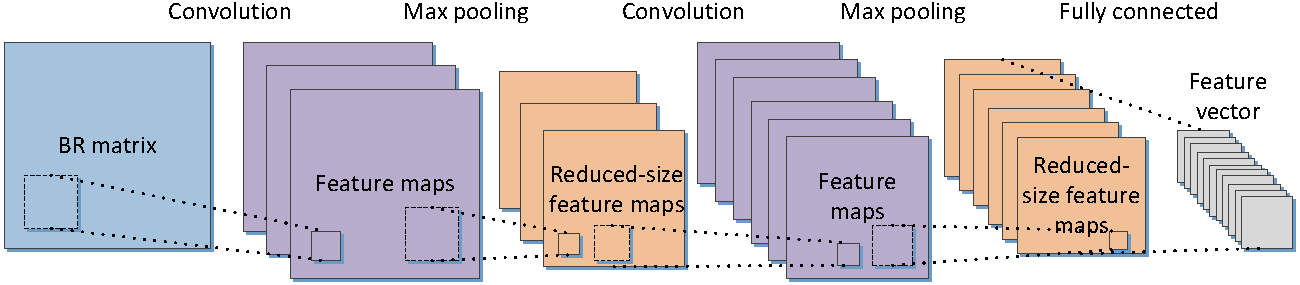
\includegraphics[width=\columnwidth]{figures/cnn.pdf}
\caption{Bug-report classification architecture: using CNN.}
\label{fig:cnn}
\end{figure}

Figure~\ref{fig:cnn} shows the overall architecture of using CNN for bug report classification. In this paper, we use a CNN with two convolutioan layers with max poolings followed by two fully connected layers with \textit{sigmoid} the activation function. It takes as input a bug report matrix $\mathcal{M} \in \mathbb{R}^{100x100}$ as described in Section~\ref{sec:bug report matrix}. The first convolutional layer uses eight fixed-size (5x5) filters to perform convolution operations over the input matrix and outputs the same number of \textit{feature maps}. A max pooling layer reduces the size of the feature maps by subsampling. The second convolutional layer using sixteen filters takes as input the output of the first layer. The fully connected layers (with fan-out of 512 and 2 respectively) project the sixteen feature maps from the second convolutional layer to a vector that serves as input to the Softmax model for computing the probability distribution.

We use the same training procedure as discussed in Section~\ref{sec:model training} to train the models (CNN and Softmax) by minimzing the cross-enropy cost function per mini-batch over a maximum 500 epochs with an early stopping criterion. 

\subsection{Multilayer Perceptron for Bug Report Classification}
\label{sec:perceptron}
A multilayer perceptron is a feedforward neural network that projects data from the input layer to a linear separable space through multiple hidden layers with activation functions \cite{Hornik:1989:MFN:70405.70408}.

\begin{equation}
  f_1(\mathbf{x}) = G_1(\mathbf{W}_1\mathbf{x} + \mathbf{b}_1), \:\: f_2(\mathbf{x}) = G_2(\mathbf{W}_2 f_1(\mathbf{x}) + \mathbf{b}_2), \:\: ...
\label{eq:perceptron}
\end{equation}

Given input $\mathbf{x}$, the output $f_i(\mathbf{x})$ of the $i^{th}$ hidden layer is shown in Equation~\ref{eq:perceptron}, where $\mathbf{W}_i$ and $\mathbf{b}_i$ are the weights matrix and bias, $G_i$ is the activation function.

We use a multilayer perceptron with three hidden layers all using 500 computation nodes and \textit{sigmoid} the activation function. A bug report matrix $\mathcal{M}$ is unpacked to a vector that serves as input to the first hidden layer. The output of the last hidden layer is fed into a fully connected layer followed by a softmax model to estimate the categorical probabilities.

The models are trained by minimizing the cross-entropy function using the same training scheme as discussed in the previous sections.

\subsection{A Simple Baseline Approach for Bug Report Classification}
\label{sec:simple baseline}
We build a simple baseline approach for bug report classification based on a simple assumption that longer content of a report contains more helpful information related to the bug.

\begin{figure}[ht]
\begin{center}
\fbox{\parbox{7.5cm}{
\textbf{def} \textcolor{blue}{\textbf{classify}}(report, threshold):\\
\hspace*{1.5em} get the bag-of-words of the report\\
\hspace*{1.5em} set $n$ = $|$bag-of-words$|$\\
\hspace*{1.5em} \textbf{if} $n$ > threshold:\\
\hspace*{3.0em} \textbf{return} "\textcolor{red}{predictable}''\\
\hspace*{1.5em} \textbf{else}:\\
\hspace*{3.0em} \textbf{return} "\textcolor{red}{unpredictable}''
}}
\caption{Classifying a bug report based on its length.}
\label{fig:simple baseline}
\end{center}
\end{figure}

The simple baseline approach is shown in Figure~\ref{fig:simple baseline}. If the length of a bug report is greater than a given threshold value, we deem it ``predictable'', otherwise, ``unpredictable''.

Unlike the neural-network approaches taking as input a bug report matrix created using word embeddings, this simple baseline approach uses the raw report as input. Although it does not learn any lexical or semantic meanings, it catches a simple but important structural information: the report size. This simple approach is general enough, as a comparison baseline, to work on any types of reports.

\begin{table*}[t]
\centering
\caption{Benchmark Projects: {bug reports are split into a testing, a validation and a training set.}}
\begin{tabular}{|c|c|c|c|c|c|c|} \hline
Project&Time Range&\# reports for testing &\# reports for validation&\# reports for training&total\\ \hline
Eclipse Platform UI &2001-10 -- 2014-01&1,156&500&2,000&3,656\\ \hline
SWT&2002-02 -- 2014-01&817&500&1,500&2,817\\ \hline
JDT&2001-10 -- 2014-01&632&500&1,500&2,632\\ \hline
\end{tabular}
\label{tab:dataset}
\end{table*}

\section{Evaluation}
\label{sec:evaluation}

This section discusses a set of extensive experiments to evaluate the effectiveness of the LSTM-based bug report classification approach on the bug locating task. Generally, we want to see whether this approach is able to filter out unhelpful bug reports to an IR-based system, whether it helps improve the bug-locating performance, what is the trade-off between precision and recall, and what is the difference in terms of performance between using different classification models.

\subsection{IR-based Bug Locating System}
\label{sec:bug locating system}
We use a recent bug locating system provided by Ye et al. \cite{Ye:ICSE16} in our experiments because: 1) it is an IR-based system; 2) it can be acquired; 3) it provides comparably good results with other state-of-the-art systems \cite{7372035, 7961519}. This system uses a \textit{\textbf{L}earning-to-\textbf{R}ank} technique combining \textbf{W}ord-\textbf{E}mbedding-based features and VSM-based features for bug locating. We denote it as LRWE in this paper.

\subsection{Benchmark Datasets}
\label{sec:benchmark dataset}
We use the same benchmark dataset with \cite{Ye:FSE14, Ye:ICSE16, 7372035, 7961519, 7832908} as shown in Table~\ref{tab:dataset}. Totally 9,105 bug reports and the corresponding source code packages from Eclipse Platform UI, SWT, and JDT are checkout and used in our experiments. We split these bug reports into a training dataset for training the classification models, a validation dataset for checking whether the models are converged or not, and a testing dataset for providing the testing result.

\subsection{Labeling the Data}
\label{sec:labeling the data}
Data labeling provides the ground truth for the experiments. The goal of our bug report classification is to filter out unhelpful bug reports while keeping the helpful ones to an IR-based bug locating system for improving locating performance and reducing false positives. So the assessment of a bug report's helpfulness (``preictable'' or ``unpredictable''), instead of being done manually, should be performed automatically by the IR-based system used in the experiments.

We perform data labeling by running the chosen bug locating system LRWE for all the bug reports. More specifically, for every bug report, we run LRWE on the corresponding source code package checked out from a commit right before its fix commit. The output of the system is a ranked list of all the source code files, from which we label the bug report as ``precitable'' to the system if at least one buggy file can be seen within the top $N$ positions. Otherwise, if the top $N$ files in the ranked list are all irrelevant files, we label the bug report as ``unpredictable''. According to Miller's $7\pm2$ law \cite{mil56}, humans are able to handle seven plus or minus two tasks simultaneously. So we choose $N=10$ under the assumption that a ranked list is useful to users if a real bug locates within the top 10 recommendations.

The output of data labeling is a set of 9,105 bug reports labeled as either ``predictable'' or ``unpredictable'' as the ground truth.

\subsection{Evaluation Metrics}
\label{sec:evaluation metrics}
We evaluate our bug report classification approach from two perspectives. First, we want to test its classification performance. Second, we want to test if it can help improve the IR-based bug locating system's ranking performance. So we run experiments using the following evaluation metrics:
\begin{itemize}
	\item \textit{true positive}: a ``predictable'' bug report that is also classified as ``predictable''
	\item \textit{false positive}: an ``unpredictable'' bug report that is classified as ``predictable''
	\item \textit{true negative}: an ``unpredictable'' bug report that is also classified as ``unpredictable''
	\item \textit{false negative}: a ``predictable'' bug report that is classified as ``unpredictable''
	\item \textit{\textbf{Accuracy}}: a standard metric measuring the correctness of the classification results.
  	\begin{equation}
		Accuracy = {|\text{true positives}| + |\text{true nagatives}| \over {\text{the totaly number of instances}}} 
	\end{equation}
   	\item \textit{\textbf{Precision}}: a standard metric measuring the usefulness of the classification results.
  	\begin{equation}
		Precision = {|\text{true positives}| \over {|\text{true positives}| + |\text{false positives}|}} 
	\end{equation}
   	\item \textit{\textbf{Recall}}: a standard metric measuring the completeness of the classification results.
  	\begin{equation}
		Recall = {|\text{true positives}| \over {|\text{true positives}| + |\text{false negatives}|}} 
	\end{equation}
	\item \textit{\textbf{F-Measure}}: a standard metric combining both Precision and Recall to measure the classification performance.
  	\begin{equation}
		F\text{-}Measure = (1 + \beta) \cdot {{Precision \cdot Recall} \over {\beta^2 \cdot Precision + Recall}} 
	\end{equation}
	When we give equal weights to Precision and Recall by setting $\beta=1$, we have \textbf{F1-Measure} that is called the harmonic mean of Precision and Recall.\\
	When we give more weights to Precision by setting $\beta=0.5$, we have \textbf{F0.5-Measure} that considers Precision is more important.
   \item \textit{Mean Average Precision (\textbf{MAP})}: a standard metric measuring the overall ranking performance of an IR system \cite{Manning:2008:IIR:1394399}. It is defined as the mean of the average precision over all queries. MAP is widely used in measuring the ranking performance of IR-based bug locating systems \cite{Huo:2017:EUF:3172077.3172153, Huo:2016:LUF:3060832.3060845, 7372035, Saha:2013:ASE:6693093, Ye:FSE14, Ye:ICSE16, Zhou:2012:BFM:2337223.2337226}.
   \item \textit{Mean Reciprocal Rank (\textbf{MRR})}: a metric measuring the ranking performance of an IR system on the first recommendation \cite{Voorhees99thetrec-8}.
\end{itemize}

We use Accuracy, Precision, Recall, F1-Measure and F0.5-Measure to evaluate the bug report classification results. We use MAP and MRR to measure the IR system's ranking results.

\subsection{Training and Testing Procedure}
\label{sec:training and testing procedure}
As discussed in Section~\ref{sec:model training}, the models are trained over a maximum 500 epochs with an early stopping criterion.

\begin{figure}[ht]
\begin{center}
\fbox{\parbox{7.5cm}{
max\_epochs = \textcolor{red}{500}\\
patience = \textcolor{red}{10}\\
best\_accuracy = \textcolor{red}{0}\\
prior\_accuracy = \textcolor{red}{0}\\
\textbf{for}(epoch = \textcolor{red}{0}; epoch \textcolor{blue}{<} max\_epoch; epoch++):\\
\hspace*{1.5em} train the model over all the batches in one cycle\\
\hspace*{1.5em} run the model on the validation set\\
\hspace*{1.5em} \textbf{if} $Accuracy$ \textcolor{blue}{>} best\_accuracy:\\
\hspace*{3.0em} best\_accuracy = $Accuracy$\\
\hspace*{3.0em} test the model on the testing set\\
\hspace*{3.0em} patience = \textcolor{red}{10}\\
\hspace*{1.5em} \textbf{else if} $Accuracy$ \textcolor{blue}{>} prior\_accuracy:\\
\hspace*{3.0em} patience = \textcolor{red}{10}\\
\hspace*{1.5em} \textbf{else}:\\
\hspace*{3.0em} patience = patience - \textcolor{red}{1}\\
\hspace*{3.0em} \textbf{if} patience \textcolor{blue}{<} \textcolor{red}{0}:\\
\hspace*{4.5em} \textbf{return} the testing results\\
\hspace*{1.5em} prior\_accuracy = $Accuracy$\\
test the model on the testing set\\
\textbf{return} the testing results
}}
\caption{The training and testing procedure.}
\label{fig:training procedure}
\end{center}
\end{figure}

Figure~\ref{fig:training procedure} shows the details of our training and testing procedure. When the models are trained over every epoch, we test the models on the validation dataset and keep track of the performance. If a continuous decrease of the validation Accuracy is observed over 10 times, we assume the models are converged and stop the training process. At the end, we report the results on the testing dataset when the models produce the best validation Accuracy.

\subsection{Tuning the Hyperparameters}
\label{sec:tuning parameters}
We tune models' hyperparameters on the validation dataset using the the same procedure as shown in Figure~\ref{fig:training procedure} but without testing on the testing set.

For LSTM-network, the number of hidden units in the memory cell is set to 32, the dropout rate on the input layer is 0.9, the output dropout rate is 0.7, and the learning rate 0.003.

For CNN, the first convolutional layer uses eight filters with size 5x5. The second convolutional layer uses sixteen 5x5 filters. The pooling size is 2x2. The fan-out of the first fully connected layer is 512.

For multilayer perceptron, all three hidden layers use 500 internal nodes.

The learning rates for both CNN and perceptron are 0.001. The training batch size for these three models are all set to 64.

The length thresholds of the simple baseline approach are chosen based on its performance on the validation set as well. Specifically, we set the thresholds to be 7,6,7 for the three benchmark projects respectively.

\subsection{Results and Analysis}
\label{sec:results and analysis}
The rest of this section reports results to answer the following research questions.
\begin{enumerate}
  \item[\textit{RQ1:}] Can the LSTM-network approach, compared with using other classification models, helps filter out ``unpredictable'' bug reports?
  \item[\textit{RQ2:}] Can the LSTM-network approach helps improve the ranking performance of the IR-based system on bug locating?
  \item[\textit{RQ3:}] Can we futher increase the Precision? If so, what is the trade-of betwen Recall?
\end{enumerate}

\subsubsection{\textbf{RQ1:}}
\label{sec:research question 1}
\textit{Can the LSTM-network approach, compared with using other classification models, helps filter out ``unpredictable'' bug reports?}

\begin{table}[ht]
\centering
\caption{Classification results of using difference models: MLP refers to the multilayer perceptron model, SB refers to the simple baseline approach, and NC (No Classification) refers to classifying all the instances (bug reports) as positive (``predictable'').}
\begin{adjustbox}{width=0.47\textwidth}
\begin{tabular}{|c|c|c|c|c|c|c|c|c|} \hline
Project & Metric & LSTM & CNN & MLP & SB & NC\\
& & & & & &\\ \hline
Eclipse & Accuracy & \textbf{0.670} & 0.650 & 0.645 & 0.658 & 0.658\\
Platform & Precision & \textbf{0.703} & 0.672 & 0.676 & 0.672 & 0.658\\
UI & Recall & 0.862 & 0.901 & 0.884 & 0.939 & \textbf{1}\\
& F1-Measure & 0.775 & 0.770 & 0.766 & 0.783 & \textbf{0.794}\\
& F0.5-Measure & \textbf{0.730} & 0.708 & 0.709 & 0.712 & 0.706\\ \hline
SWT & Accuracy & \textbf{0.694} & 0.685 & 0.692 & 0.659 & 0.692\\
& Precision & 0.694 & 0.698 & 0.692 & \textbf{0.700} & 0.692\\
& Recall & \textbf{1} & 0.963 & 0.884 & 0.887 & \textbf{1}\\
& F1-Measure & \textbf{0.819} & 0.809 & 0.783 & 0.783 & 0.818\\
& F0.5-Measure & \textbf{0.739} & 0.738 & 0.738 & 0.731 & 0.738\\ \hline
JDT & Accuracy & \textbf{0.763} & 0.747 & 0.710 & 0.737 & 0.759\\
& Precision & \textbf{0.762} & 0.761 & 0.758 & 0.761 & 0.759\\
& Recall & \textbf{1} & 0.971 & 0.908 & 0.952 & \textbf{1}\\
& F1-Measure & \textbf{0.865} & 0.853 & 0.823 & 0.846 & \textbf{0.863}\\
& F0.5-Measure & \textbf{0.8} & 0.796 & 0.784 & 0.793 & 0.797\\ \hline
\end{tabular}
\end{adjustbox}
\label{tab:classification results}
\end{table}

To answer the first research question, we run different classification models on three benchmark projects. The results are shown in Table~\ref{tab:classification results}, where each column shows the results of a model on different projects.

We obtain the following observations from the results: (1) Compared with not doing bug report classificationusing, using the LSTM-network approach helps (as Precision increases) filter out ``unpredictable'' reports. (2) While the LSTM-network increases the classification precision, it drops the recall. It helps reduce false positives but also reduce true positives. (3) Using LSTM-network can increase F0.5-Measure but may decrease F1-Measure. If we consider Precision and Recall are equally important, LSTM may not help. But if we prefer precision over recall under a certain trade-off (F0.5-Measure), using LSTM-network helps. (4) Using LSTM-network achieves better classification performance than using CNN, multilayer perceptron, and the simple baseline approach. It shows that the long-term dependencies learned by LSTM is useful to decide the usefulness of a bug report to IT-based bug locating. (5) Interestingly, the simple baseline approach provides comparable performance with CNN and multilayer perceptron. One potential reason may be because the content size of a report is more important than the locality dependencies of the bug report matrix. (6) We also observe that the performane difference between LSTM and other models on SWT and JDT, compared with on Eclipse, are marginal. One potential reason may be the smaller training size and testing size. But it still produces better precisions while even keeping the same F1-Measure and better F0.5-Measure on these two projects.

Overall, the LSTM-network shows better results on the three benchmark projects especially on Eclipse Platform UI. So we answer \textit{RQ1} that the LSTM-network approach helps filter out ``unpredictable'' bug reports under a certain trade-off (F0.5-Measure) between recall.

\subsubsection{\textbf{RQ2:}}
\label{sec:research question 2}
\textit{Can the LSTM-network approach helps improve the ranking performance of the IR-based system on bug locating?}

\begin{table}[ht]
\centering
\caption{Bug locating results: SB refers to the simple baseline approach, NC (No Classification) refers to classifying all the instances (bug reports) as positive (``predictable'').}
\begin{adjustbox}{width=0.43\textwidth}
\begin{tabular}{|c|c|c|c|c|c|c|} \hline
Project & Metric & LSTM & SB & NC\\
& & & &\\ \hline
Eclipse & MAP & \textbf{0.405} & 0.382 & 0.369\\
Platform & MRR & \textbf{0.460} & 0.432 & 0.419\\
UI & Recall & 0.862 & 0.939 & \textbf{1}\\
& F0.5-Measure & \textbf{0.730} & 0.712 & 0.706\\ \hline
SWT & MAP & 0.383 & \textbf{0.393} & 0.382\\
& MRR & 0.444 & \textbf{0.455} & 0.443\\
& Recall & \textbf{1} & 0.887 & \textbf{1}\\
& F0.5-Measure & \textbf{0.739} & 0.731 & 0.738\\ \hline
JDT & MAP & \textbf{0.430} & 0.425 & 0.425\\
& MRR & \textbf{0.521} & 0.520 & 0.516\\
& Recall & \textbf{1} & 0.952 & \textbf{1}\\
& F0.5-Measure & \textbf{0.8} & 0.793 & 0.797\\ \hline
\end{tabular}
\end{adjustbox}
\label{tab:ranking results}
\end{table}

To test whether our approach helps improve the IR-based system on bug locating, we apply our LSTM-based model on bug reports in the testing dataset and run the IR-beased bug locating system LRWE on only the ``predictable'' reports. Table~\ref{tab:ranking results} shows the comparison results with not doing bug report classification. We observed an obvioius performance improvement in terms of MAP and MRR over both the simple baseline approach and not doing classification on Eclipse Platform UI. For SWT the JDT, like in Table~\ref{tab:ranking results}, the advantage is not obvious. It may caused by the smaller training and testing size. We leave it to future work to collect more data and perform more fine-grained tuning of these two projects. To save time, we do not run experiments on CNN and multilayer perceptron because they do not show comparable classification performance with LSTM in the preivious section.

Our answer to \textit{RQ2} is that the LSTM-network approach, under the trade-off (F0.5-Measure) between recall, helps improve the IR-based bug location system's ranking performance.

\subsubsection{\textbf{RQ3:}}
\label{sec:research question 3}
\textit{Can we futher increase the Precision? If so, what is the trade-of between Recall?}

As discussed in Section~\ref{sec:categorical distribution}, a bug report is classified to a category based on its categorical probabilities, which are computed as output by the Softmax model. That is, based on the output of Softmax, we classify a report as ``predictable'' when $P(``predictable'') > P(``unpredictable'')$ even the difference is marginal.

To further increase the classification precision, instead of classifying a report to the category with larger probability, we perform classification using a fixed value as the threshold. That is, we classify a bug report as ``predictable'' if $P(``predictable'') > threshold$ and ``unpredictable'' otherwise. Our assumption is that the bigger threshold the more confidence of the model in classifying a report as ``predictable''.

We run experiments using different classification models on the Eclipse Platform UI project by tuning the probability threshold from 0 to 1. For the simple baseline approach, we tune the length as the the threshold. Then we draw a learning curve for each evaluation metric. The learning curves are shown in Figure~\ref{fig:learning curve of lstm} for LSTM, Figure~\ref{fig:learning curve of cnn} for CNN, Figure~\ref{fig:learning curve of perceptron} for multilayer perceptron, and Figure~\ref{fig:learning curve of simple baseline} for the simple baseline approach.

An overall observation from the results is that the precision increases when we increase the threshold, but the recall drops. When we give more preference to precision, we observe that the F0.5-Measure value also increase.

More specifically, take the LSTM result shown in Figure~\ref{fig:learning curve of lstm} for example, both Precision and F0.5-Measure increase with the probability threshold. When the threshold is set to 0, which means no classifications at all, the Precision is 0.658 and the F0.5-Measure is 0.706. After we increase the threshold to 0.5, we obtain the result shown in Table~\ref{tab:classification results}, where Precision is 0.703 and F0.5-Measure is 0.73. Then we continue to increase the probability threshold. When the threshold increases to 0.8, which means that we classify a bug report as ``predictable'' only when $P(``predictable'') > 0.8$, the Precision also increases from 0.703 to 0.716, and the F0.5-Measure increases from 0.73 to 0.735.

Next, to get more insights into the difference between models, we compare the changes of precision over the changes of recall in Figure~\ref{fig:precision vs recall}, from which we clearly observe that the LSTM-network (RNN) model achieves better performance in terms of Precision than other models before the Recall drops too much. We also observe that CNN gives better Precision when Recall drops below 0.5 that is too low to be useful.

In summary, we answer \textit{RQ3} that we can further increase the Precision while keeping a certain trade-off (in terms of F0.5-Measure) between recall. The LSTM-network achieves the best trade-off between Precision and Recall.

\begin{figure}[H]
\centering
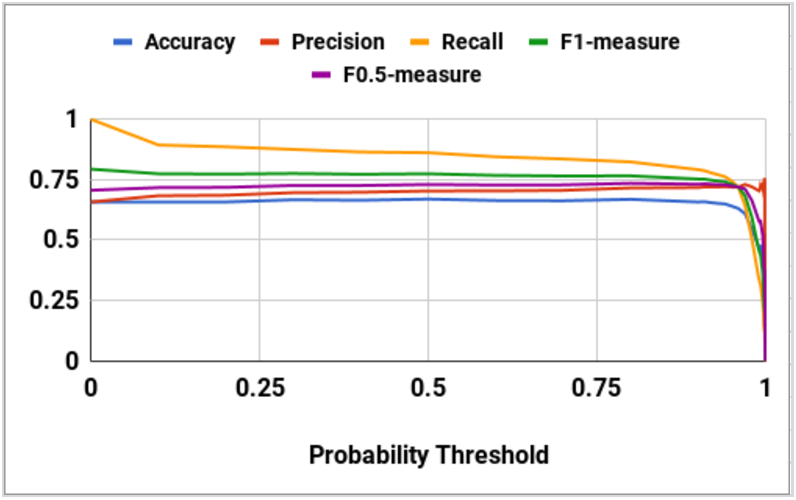
\includegraphics[scale=0.58]{figures/result_rnn1.pdf}
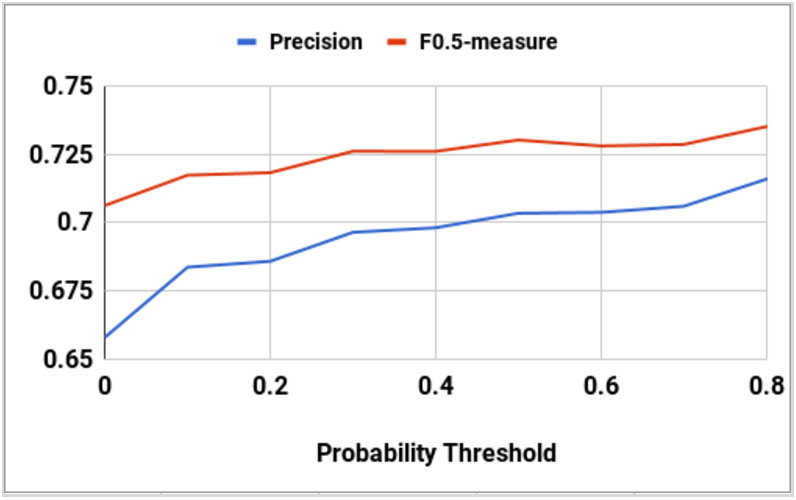
\includegraphics[scale=0.58]{figures/result_rnn2.pdf}
\caption{Learning curves for LSTM.}
\label{fig:learning curve of lstm}
\end{figure}
\begin{figure}[H]
\centering
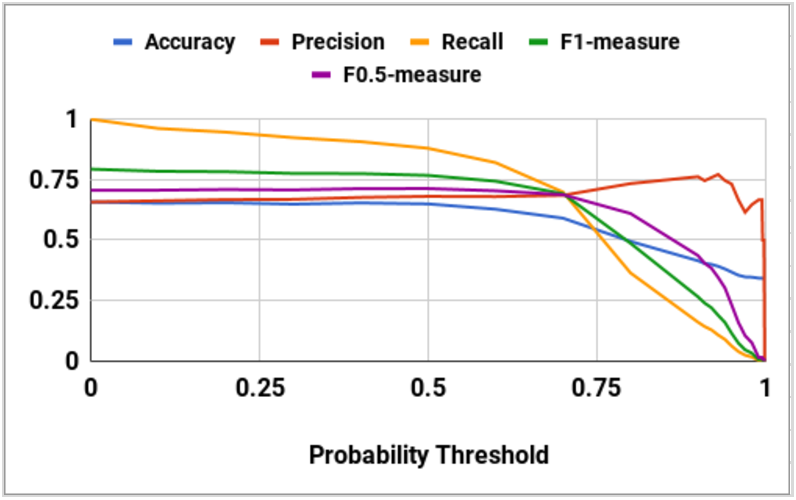
\includegraphics[scale=0.58]{figures/result_cnn1.pdf}
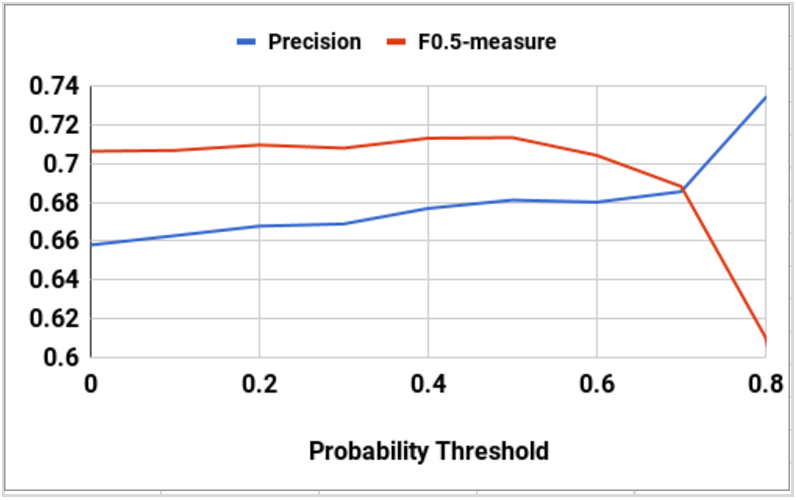
\includegraphics[scale=0.58]{figures/result_cnn2.pdf}
\caption{Learning curves for CNN.}
\label{fig:learning curve of cnn}
\end{figure}
\begin{figure}[H]
\centering
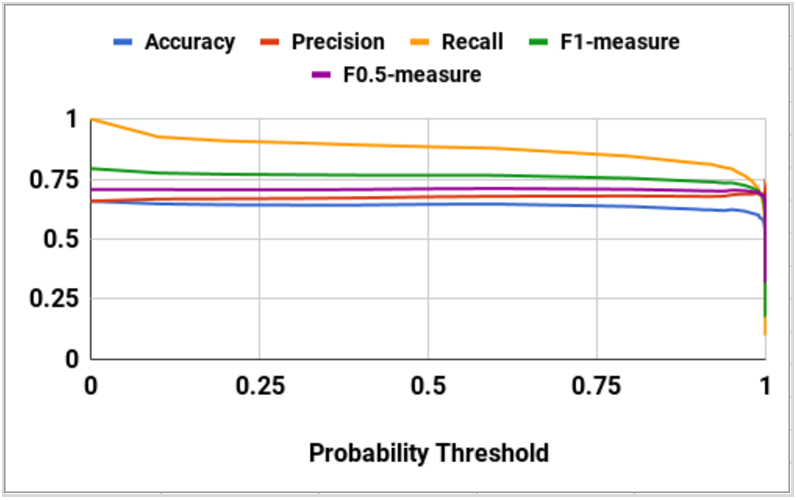
\includegraphics[scale=0.58]{figures/result_perceptron1.pdf}
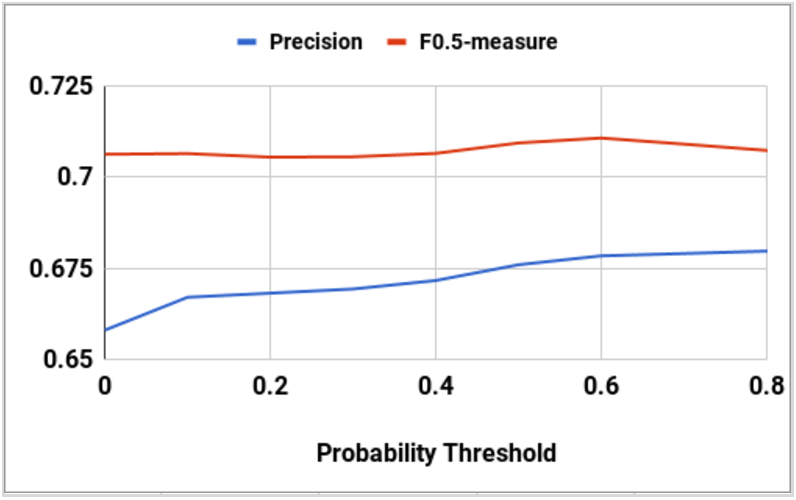
\includegraphics[scale=0.58]{figures/result_perceptron2.pdf}
\caption{Learning curves for multilayer perceptron.}
\label{fig:learning curve of perceptron}
\end{figure}
\begin{figure}[H]
\centering
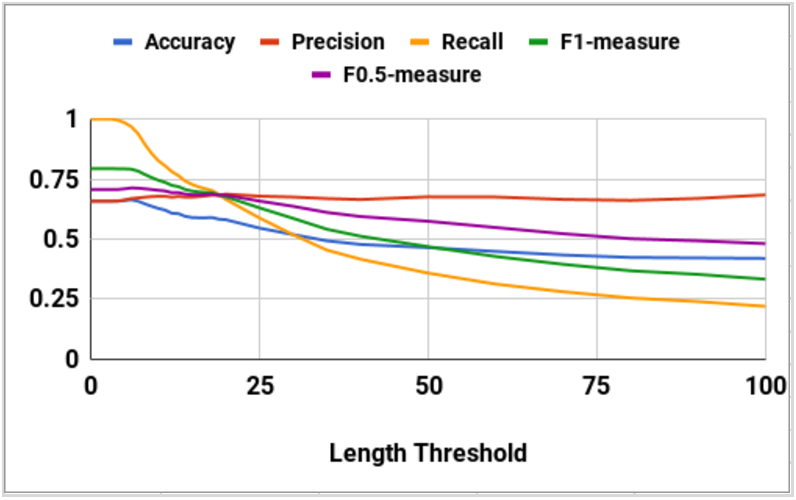
\includegraphics[scale=0.58]{figures/result_simple1.pdf}
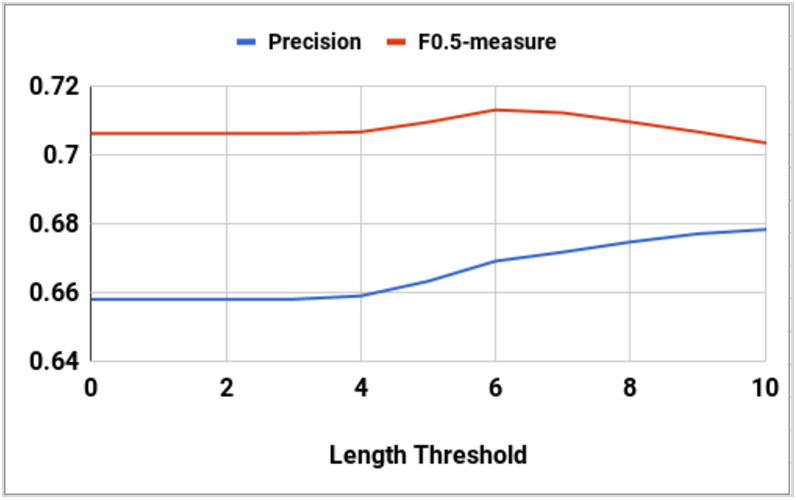
\includegraphics[scale=0.58]{figures/result_simple2.pdf}
\caption{Learning curves for the simple baseline approach.}
\label{fig:learning curve of simple baseline}
\end{figure}

\begin{figure}[H]
\centering
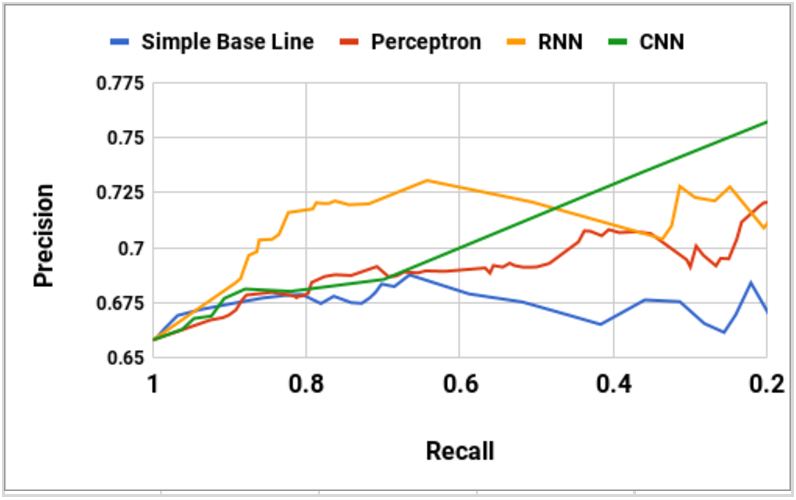
\includegraphics[width=\columnwidth]{figures/precision_recall.pdf}
\caption{Precision vs. Recall.}
\label{fig:precision vs recall}
\end{figure}

